\section{Dataset Description}
\label{sec:dataset}

This study utilizes a curated X-ray diffraction (XRD) pattern dataset derived from the American Mineralogist Crystal Structure Database (AMCSD). The dataset comprises paired experimental and simulated XRD patterns for mineral identification and classification tasks.

\subsection{Dataset Composition}

The dataset contains 13,325 XRD patterns representing 3,962 unique mineral classes. Each pattern consists of 4,500 intensity values spanning a $2\theta$ range of 5--90$^\circ$, providing comprehensive coverage of the diffraction angles typically used in powder XRD analysis. Table~\ref{tab:dataset_stats} summarizes the key statistics of the dataset.


\begin{table}[htbp]
\centering
\caption{Summary statistics of the XRD dataset.}
\label{tab:dataset_stats}
\begin{tabular}{lr}
\toprule
\textbf{Property} & \textbf{Value} \\
\midrule
Total XRD patterns & 13,325 \\
Unique mineral classes & 3,962 \\
Pattern length (data points) & 4,500 \\
2$\theta$ range & 5--90$^\circ$ \\
\midrule
\multicolumn{2}{l}{\textit{Class Distribution}} \\
\midrule
Minimum samples per class & 1 \\
Maximum samples per class & 100 \\
Mean samples per class & 3.36 \\
Median samples per class & 1 \\
Classes with only 1 sample & 2,375 (59.9\%) \\
Classes with $\leq$5 samples & 3,537 (89.3\%) \\
Classes with $\geq$50 samples & 26 (0.7\%) \\
\midrule
\multicolumn{2}{l}{\textit{DTW Distance (Experimental vs. Simulated)}} \\
\midrule
Mean DTW distance & 9.33 \\
Median DTW distance & 6.15 \\
Std. deviation & 9.03 \\
Range & 0.36--100.00 \\
\bottomrule
\end{tabular}
\end{table}


\subsection{Class Distribution Analysis}

The dataset exhibits significant class imbalance, a common challenge in mineral classification. As shown in Figure~\ref{fig:class_distribution}, the distribution of samples per class is heavily right-skewed. The median number of samples per class is 1, while the mean is 3.36, indicating that most classes have very few samples while a small number of classes dominate the dataset.

Specifically, 2,375 classes (59.9\%) contain only a single sample, and 3,537 classes (89.3\%) have five or fewer samples. In contrast, only 26 classes (0.7\%) contain 50 or more samples. The most represented minerals include Iron, Periclase, Pyroxene-ideal, Pyroxene, and Spinel, each with approximately 100 samples.

\begin{figure}[htbp]
    \centering
    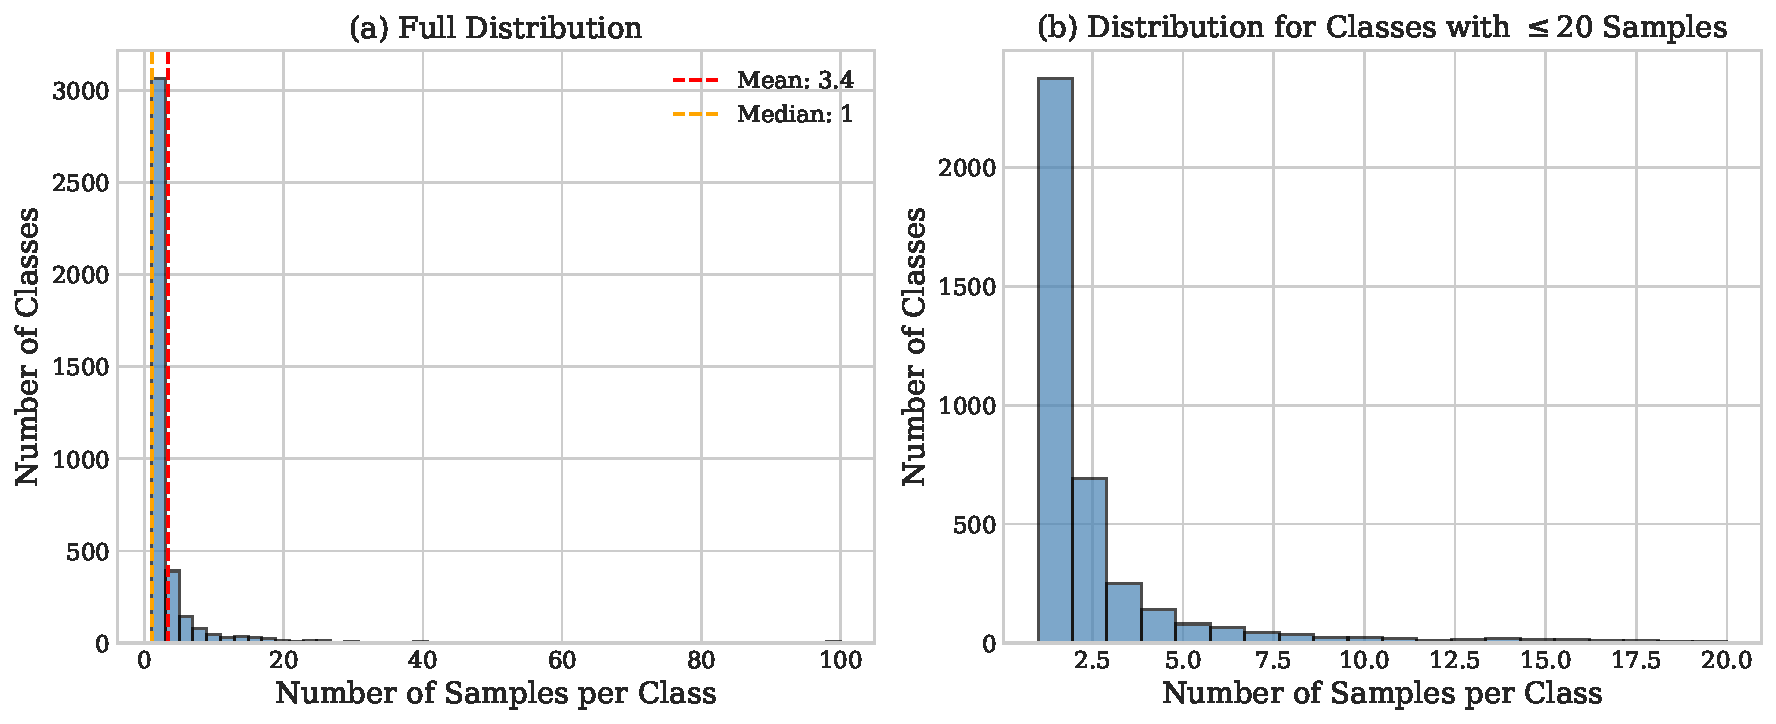
\includegraphics[width=\textwidth]{figures/class_distribution.pdf}
    \caption{Distribution of samples per mineral class. (a) Full distribution showing the extreme right-skew characteristic of the dataset. (b) Zoomed view of classes with 20 or fewer samples, highlighting that the majority of classes fall in this range.}
    \label{fig:class_distribution}
\end{figure}

\begin{figure}[htbp]
    \centering
    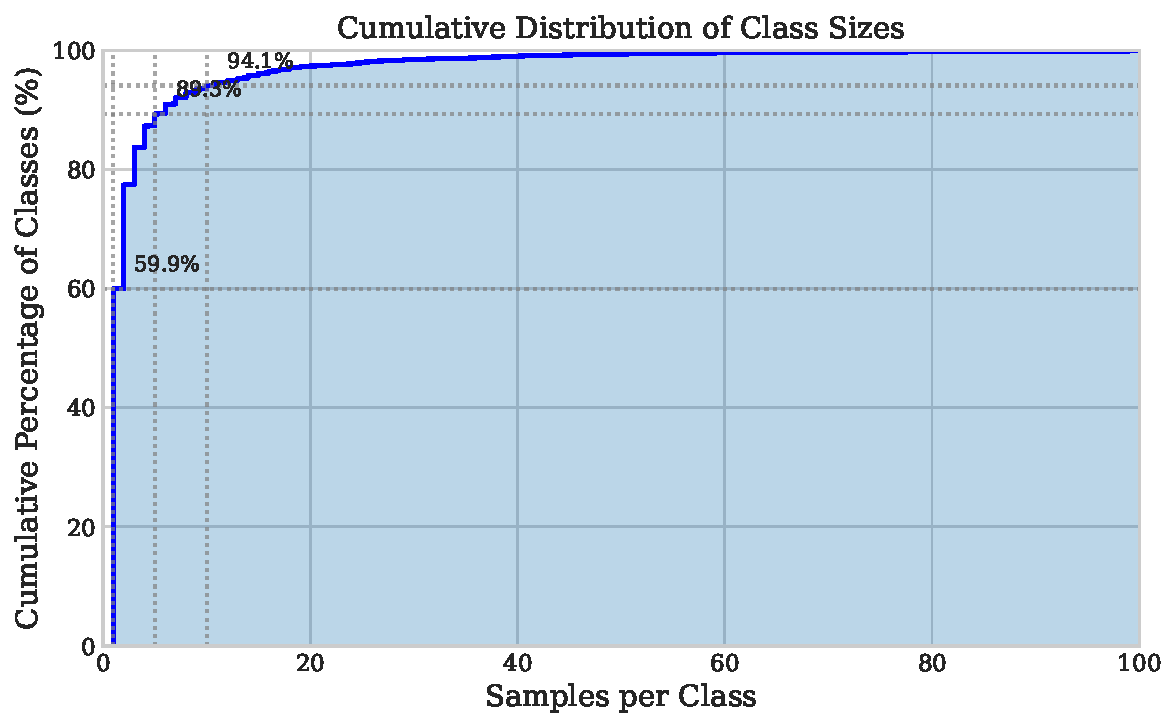
\includegraphics[width=0.7\textwidth]{figures/cumulative_distribution.pdf}
    \caption{Cumulative distribution of class sizes, showing the percentage of classes with a given number of samples or fewer.}
    \label{fig:cumulative}
\end{figure}

\subsection{XRD Pattern Characteristics}

Each entry in the dataset contains both an experimental XRD pattern and a corresponding simulated pattern calculated from the crystal structure. All patterns are normalized to have a maximum intensity of 1.0 and minimum of 0.0. Figure~\ref{fig:sample_patterns} presents representative examples of experimental-simulated pattern pairs, demonstrating varying degrees of agreement between the two.

The Dynamic Time Warping (DTW) distance metric quantifies the similarity between experimental and simulated patterns. The mean DTW distance is 9.33 with a standard deviation of 9.03 (Figure~\ref{fig:dtw_distribution}). This variation reflects factors such as preferred orientation effects, peak broadening, background contributions, and structural differences between the ideal crystal structure and real samples.

\begin{figure}[htbp]
    \centering
    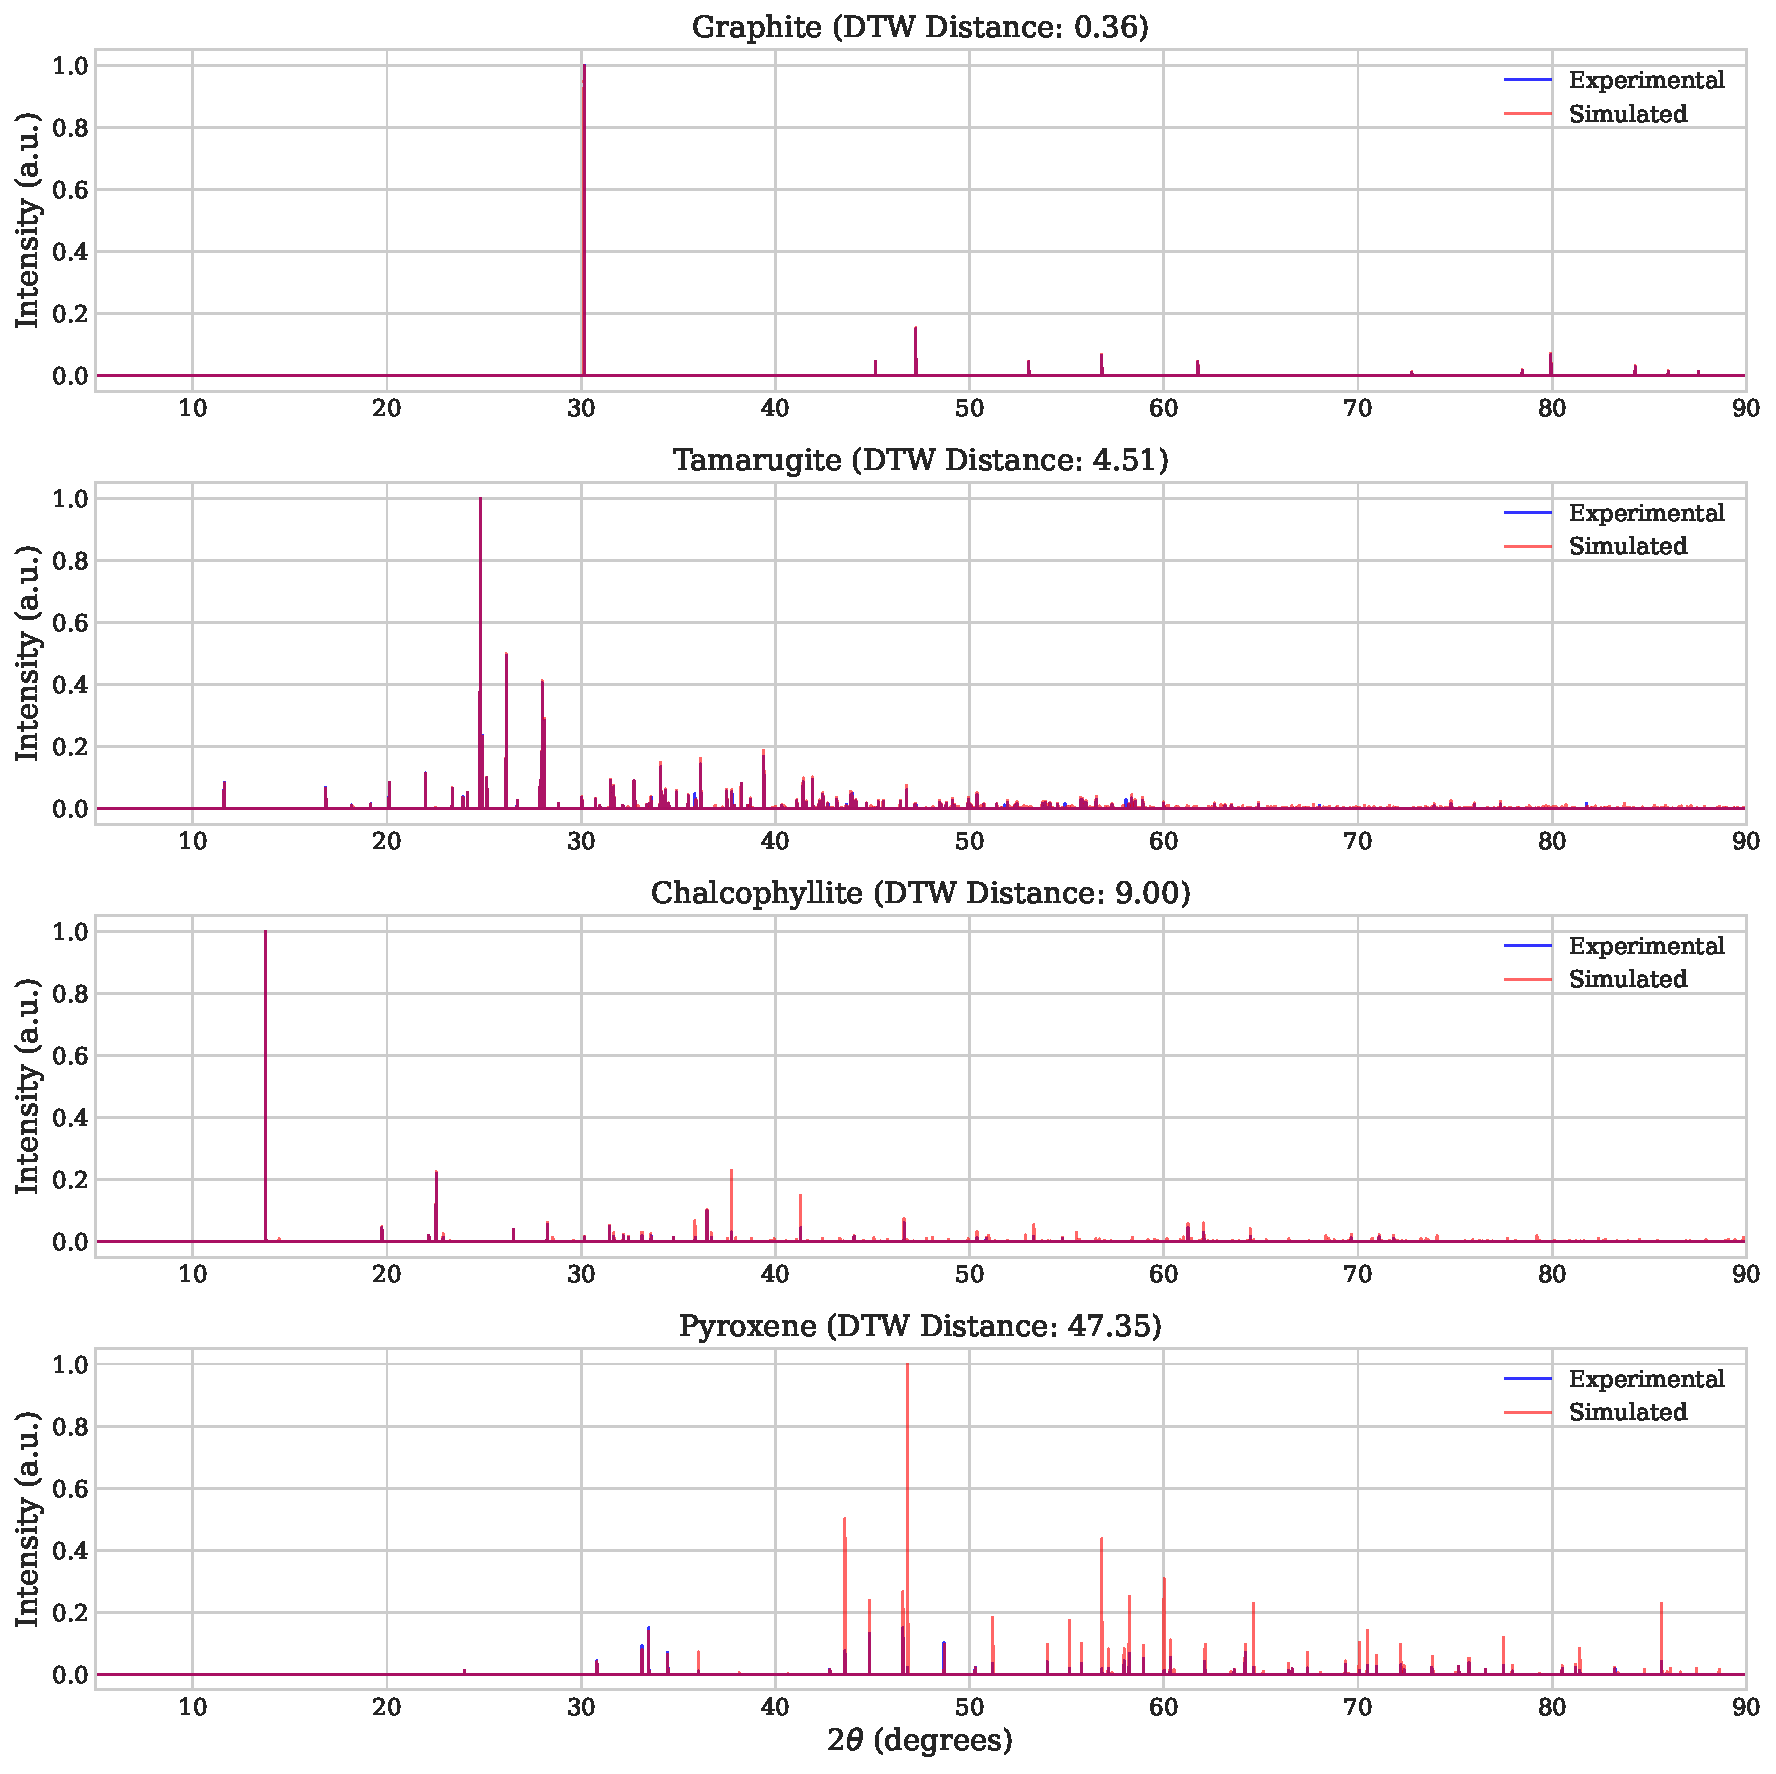
\includegraphics[width=\textwidth]{figures/sample_patterns.pdf}
    \caption{Representative XRD patterns showing experimental (blue) and simulated (red) diffraction patterns for selected minerals. The DTW distance indicates the degree of agreement between experimental and theoretical patterns.}
    \label{fig:sample_patterns}
\end{figure}

\begin{figure}[htbp]
    \centering
    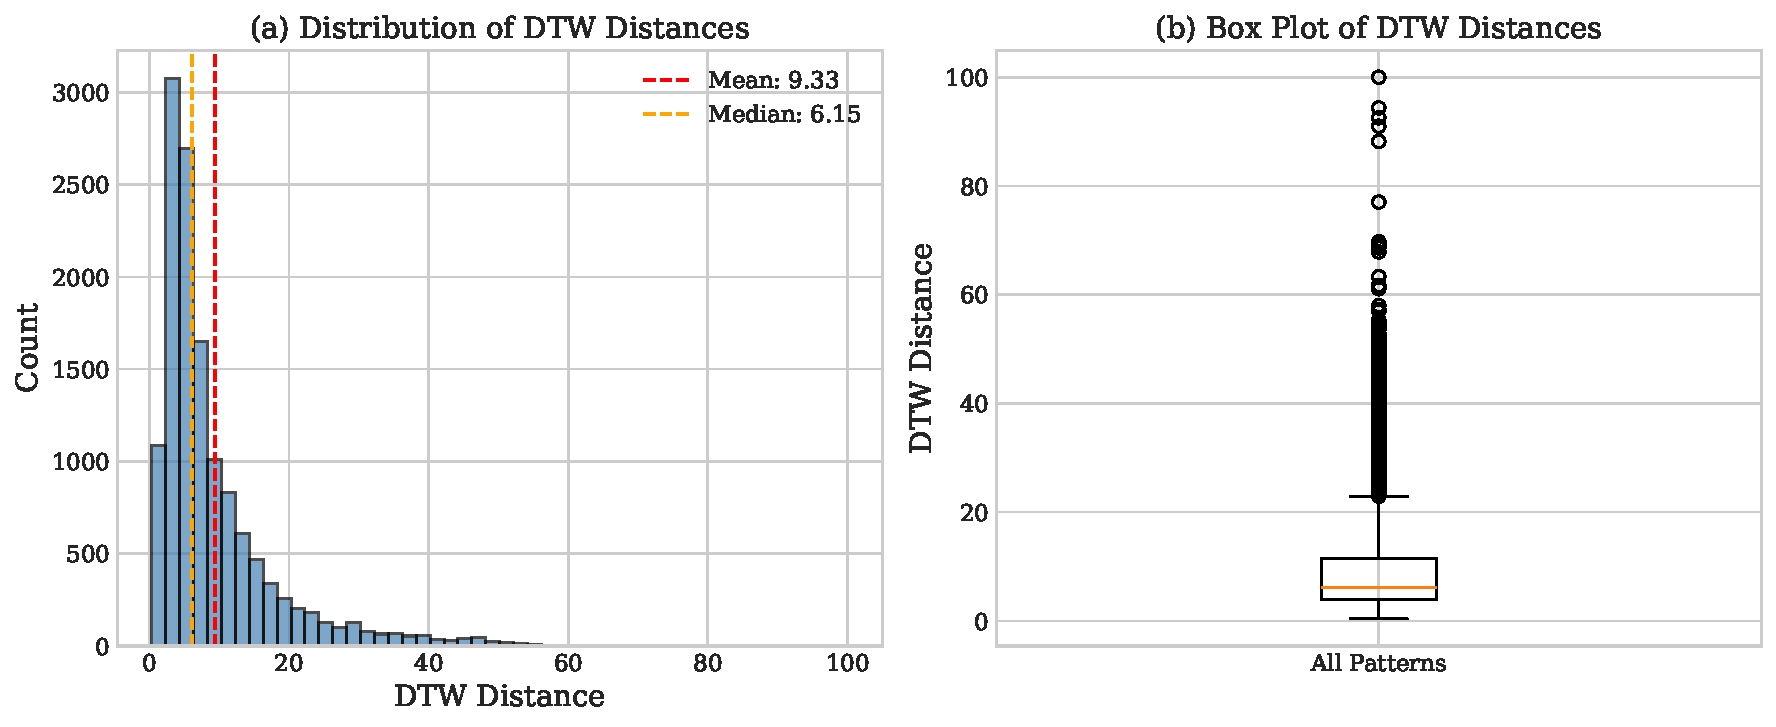
\includegraphics[width=\textwidth]{figures/dtw_distribution.pdf}
    \caption{Distribution of DTW distances between experimental and simulated XRD patterns. (a) Histogram with mean and median indicated. (b) Box plot showing the spread and outliers.}
    \label{fig:dtw_distribution}
\end{figure}

\subsection{Data Quality and Preprocessing}

The patterns in the dataset are clean, with no missing values (NaN) or infinite values detected. The intensity normalization ensures consistent scaling across all patterns, which is essential for neural network training. Figure~\ref{fig:pattern_stats} presents statistics on pattern characteristics across the dataset, including the distribution of integrated intensities and peak counts.

\begin{figure}[htbp]
    \centering
    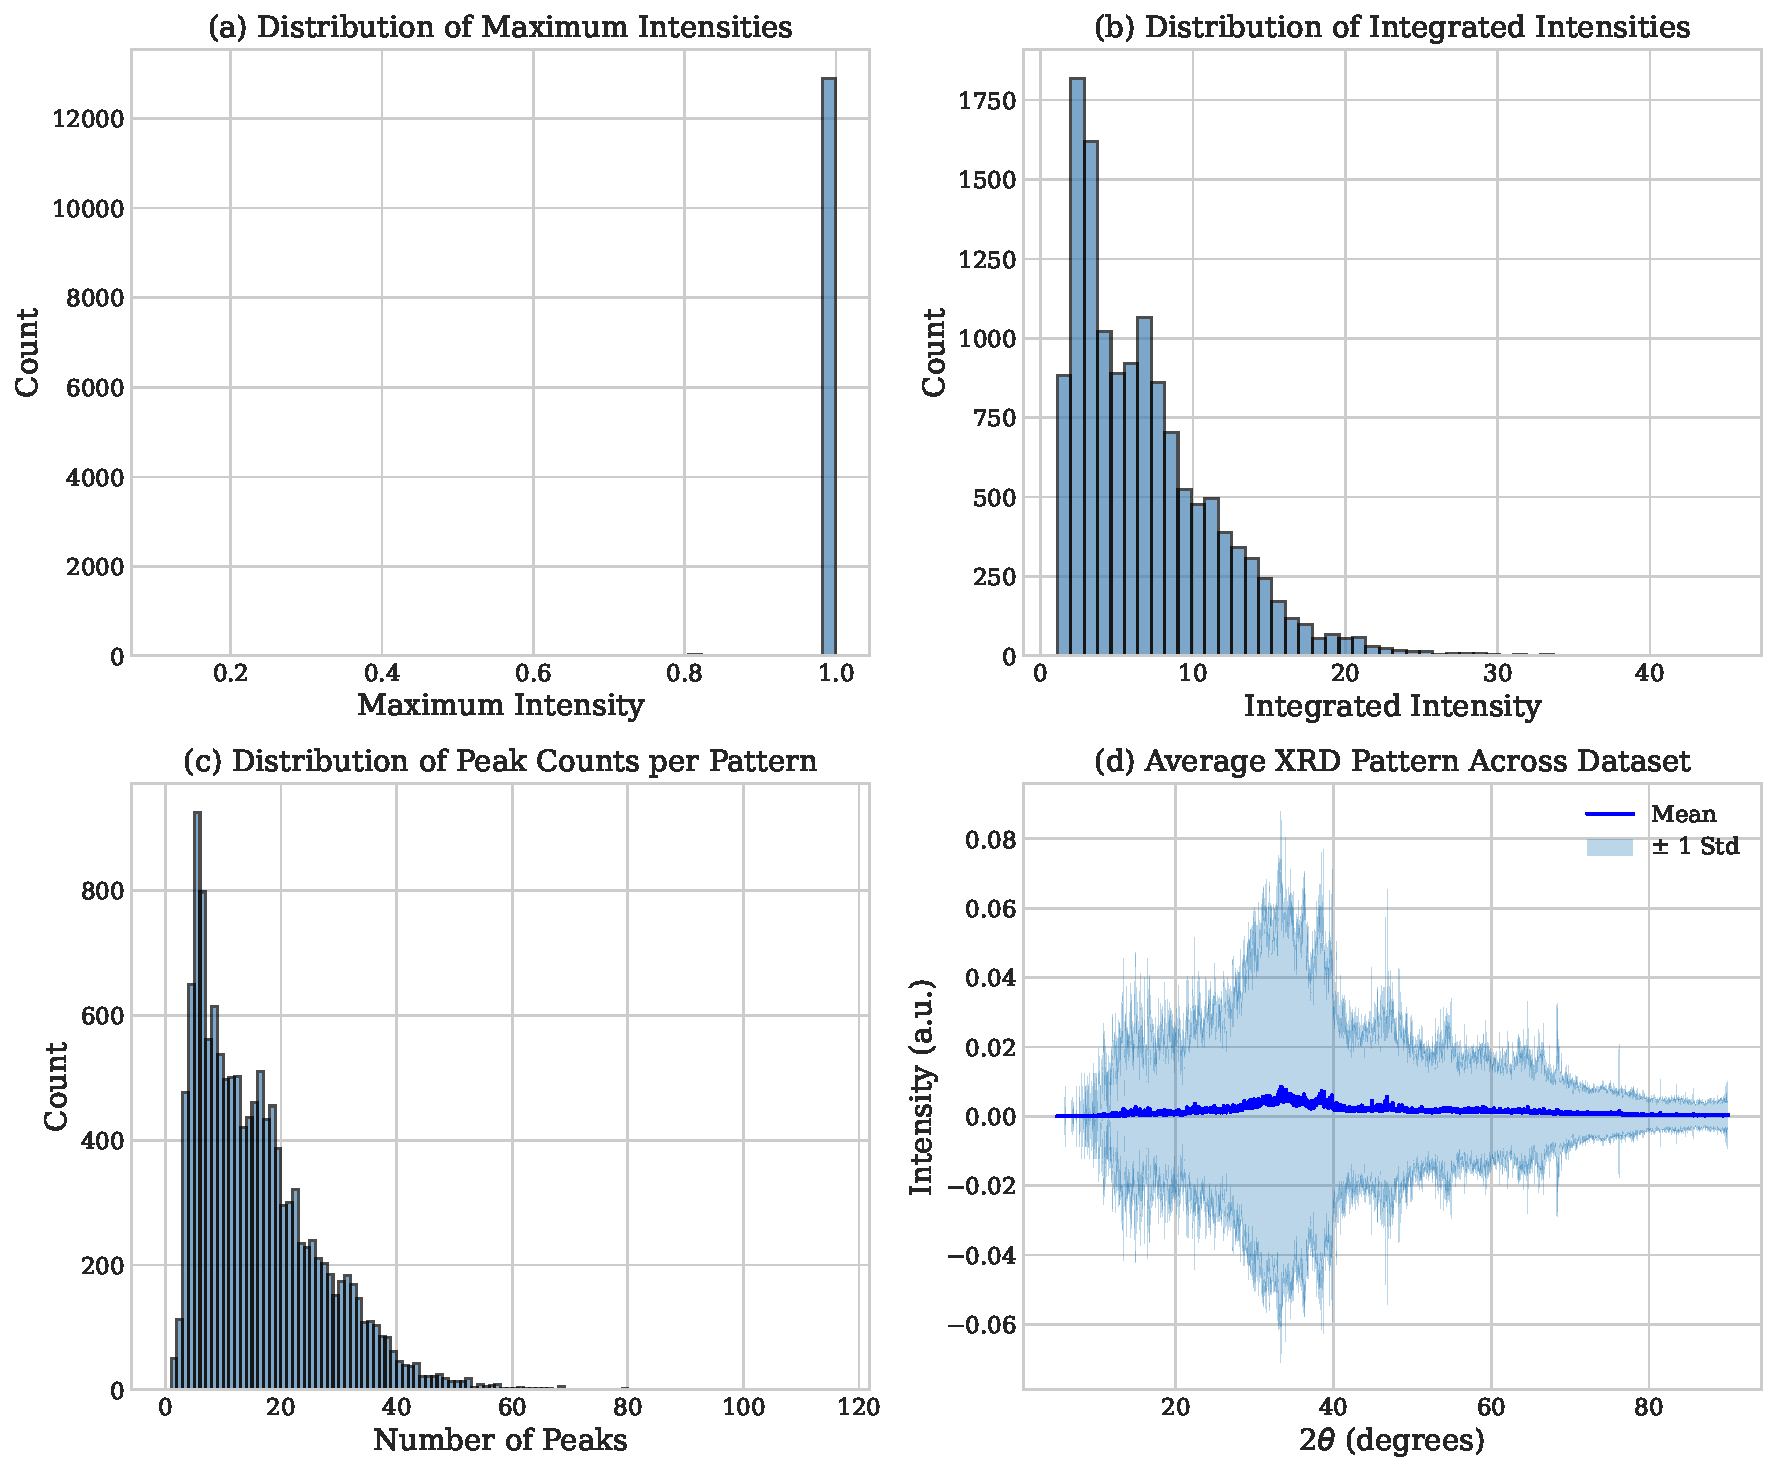
\includegraphics[width=\textwidth]{figures/pattern_intensity_stats.pdf}
    \caption{Statistical analysis of XRD pattern characteristics. (a) Distribution of maximum intensities. (b) Distribution of integrated intensities. (c) Distribution of peak counts per pattern. (d) Average XRD pattern across the entire dataset with standard deviation envelope.}
    \label{fig:pattern_stats}
\end{figure}

\subsection{Implications for Classification}

The extreme class imbalance presents significant challenges for training machine learning classifiers. Several strategies can be employed to address this:

\begin{itemize}
    \item \textbf{Data augmentation}: Generating synthetic XRD patterns using diffusion models or traditional augmentation techniques to balance the class distribution.
    \item \textbf{Few-shot learning}: Employing metric learning approaches such as Siamese networks or prototypical networks that can learn from limited examples.
    \item \textbf{Class weighting}: Applying inverse frequency weighting during training to prevent the model from being biased toward majority classes.
    \item \textbf{Hierarchical classification}: Leveraging mineralogical taxonomies to group related minerals and perform multi-level classification.
\end{itemize}

The paired experimental-simulated data also enables semi-supervised and self-supervised learning approaches, where the relationship between the two pattern types can provide additional training signal.

